% =====================================================================
%  ШАБЛОН ЛЕКЦИИ — справочник по возможностям конфига.
%  В сборку не входит. Чтобы посмотреть, как он выглядит в PDF, временно
%  добавьте в main.tex строку % =====================================================================
%  ШАБЛОН ЛЕКЦИИ — справочник по возможностям конфига.
%  В сборку не входит. Чтобы посмотреть, как он выглядит в PDF, временно
%  добавьте в main.tex строку % =====================================================================
%  ШАБЛОН ЛЕКЦИИ — справочник по возможностям конфига.
%  В сборку не входит. Чтобы посмотреть, как он выглядит в PDF, временно
%  добавьте в main.tex строку % =====================================================================
%  ШАБЛОН ЛЕКЦИИ — справочник по возможностям конфига.
%  В сборку не входит. Чтобы посмотреть, как он выглядит в PDF, временно
%  добавьте в main.tex строку \include{lectures/_template}.
%
%  Новая лекция: скопируйте этот файл в lectures/lecNN.tex, удалите лишнее,
%  замените метки tpl:... на свои (например, lec03:...).
% =====================================================================
%  Лекция NN. <Тема>
%  Дата: ГГГГ-ММ-ДД
% =====================================================================

% Короткое название в [ ] попадает в оглавление и закладки PDF,
% полное — в заголовок на странице. Если название короткое, [ ] не нужны.
\section[Шаблон лекции]{Шаблон лекции: все возможности конфига}
\label{tpl:lecture}

\subsection{Окружения}

% ---------- Нумерованные окружения (общий счётчик внутри лекции) ----------

\begin{definition}
  \emph{Статистикой} называется любая борелевская функция от выборки.
\end{definition}

% Название в [ ] печатается жирным рядом с номером.
\begin{theorem}[Гливенко--Кантелли]
  \label{tpl:glivenko}
  $\sup_{x \in \R} \abs{F_n^*(x) - F(x)} \toas 0$ \textup{при} $n \to \infty$.
\end{theorem}

\begin{lemma}
  \label{tpl:lemma}
  Если $\xi_n \toas \xi$, то $\xi_n \toP \xi$.
\end{lemma}

\begin{proposition}
  \label{tpl:xbar}
  Если $\E X_1 = \mu$ конечно, то $\Xbar \toas \mu$.
\end{proposition}

\begin{proof}
  Это усиленный закон больших чисел.
\end{proof}

\begin{corollary}
  $\Xbar \toP \mu$ (по лемме~\ref{tpl:lemma}).
\end{corollary}

\begin{example}
  Если $X_i \iid \Bern(p)$, то $\Xbar \toas p$.
\end{example}

\begin{exercise}
  Докажите, что $\E S^2 = \frac{n-1}{n}\,\sigma^2$.
\end{exercise}

% ---------- Ненумерованные ----------

\begin{remark}
  Замечание: курсивный заголовок, без номера.
\end{remark}

\begin{note}
  Примечание: то же, что замечание, другое слово.
\end{note}

% ---------- Плашки ----------

% Напоминание уже известного (серое, без номера). Заголовок можно сменить:
% \begin{reminder}[Из теории вероятностей]
\begin{reminder}
  Функция $f \colon \R^n \to \R^m$ называется \emph{борелевской}, если
  $f^{-1}(B) \in \mathcal{B}(\R^n)$ для любого $B \in \mathcal{B}(\R^m)$.
\end{reminder}

% Рамка для главного итога/формулы (синяя). Заголовок необязателен.
\begin{keybox}[Итог]
  $\Xbar$~--- несмещённая и сильно состоятельная оценка $\mu$.
\end{keybox}

% Доказательство, которое заканчивается выносной формулой:
% \qedhere ставит квадратик на строке формулы, а не ниже.
\begin{proof}[Доказательство утверждения~\ref{tpl:xbar}]
  По линейности матожидания
  \[
    \E \Xbar = \frac1n \sum_{i=1}^n \E X_i = \mu. \qedhere
  \]
\end{proof}

\subsection{Формулы}

% Строчная формула: $...$.  Выносная без номера: \[ ... \].
Строчная формула $\xi \colon \Omega \to \R$ и выносная без номера:
\[
  \P_\xi\bigl((-\infty, x]\bigr) = F(x).
\]

% С номером (номер вида (NN.k)) и меткой для ссылки:
Выносная с номером:
\begin{equation}
  \label{tpl:eq:mean}
  \Xbar = \frac{1}{n} \sum_{i=1}^{n} X_i.
\end{equation}

% Несколько строк, выровненных по & (обычно перед =). Без номеров — align*,
% с номерами — align (тогда \notag убирает номер у отдельной строки).
Несколько строк с выравниванием:
\begin{align}
  \E S^2 &= \E X_1^2 - \E \Xbar^2 \notag \\
         &= \frac{n-1}{n}\,\sigma^2. \label{tpl:eq:s2}
\end{align}

% Несколько строк по центру, без выравнивания:
\begin{gather*}
  \nu_1 + \ldots + \nu_m = n, \\
  h_i = \frac{\nu_i}{n l_i}.
\end{gather*}

% Кусочная функция. Дроби в cases маленькие; для крупных — dcases.
Кусочная функция:
\[
  \Ind{x \in A} =
  \begin{cases}
    1, & \text{если } x \in A, \\
    0, & \text{иначе}.
  \end{cases}
\]

\subsection{Ссылки}

% \cref сам подставляет слово: «теорема», «утверждение», «лекция», «рис.»...
% но ТОЛЬКО в именительном падеже. Для других падежей пишите слово сами
% и ставьте \ref (только номер): «по теореме~\ref{...}», «из леммы~\ref{...}».
% Формулы: \cref{eq} даёт «(3.1)» — подходит в любом падеже.
См. \cref{tpl:glivenko}; \cref{tpl:xbar}; \cref{tpl:ecdf}.
По теореме~\ref{tpl:glivenko} эмпирическая функция распределения сходится
равномерно. Из формул \cref{tpl:eq:mean} и~\cref{tpl:eq:s2} следует\ldots{}
Ссылка на другую лекцию: см.~\cref{lec:01}.

\subsection{Макросы обозначений}

% Полный список — в preamble/macros.tex и в таблице notation.tex.
\begin{itemize}
  \item Множества: $\R$, $\N$, $\Z$, $\mathcal{B}(\R)$.
  \item Моменты: $\P(A)$, $\E X$, $\D X$, $\Var X$, $\cov(X, Y)$, $\corr(X, Y)$, $\Ind{A}$.
  \item Модель: $\Pt$, $\Et$, $\Dt$, $\Th$, $\sample$, $\Xbar$, $\est\theta$, $X_i \iid F$.
  \item Эмпирические: $\Pemp(B)$, $F_n^*(x)$.
  \item Сходимости: $\toas$, $\toP$, $\tod$, $\toLp{2}$.
  \item Распределения: $\Norm(\mu, \sigma^2)$, $\Bern(p)$, $\Bin(n, p)$,
        $\Pois(\lambda)$, $\Exp(\lambda)$, $\Unif[a, b]$.
  \item Прочее: $a \eqdef b$, $\argmax_\theta L(\theta)$, $\abs{x}$,
        $\epsilon$ (это $\varepsilon$), $\phi$ (это $\varphi$),
        $\le$ и $\ge$ (наклонные).
\end{itemize}

\subsection{Списки}

% Нумерованный список. Метки можно менять: \begin{enumerate}[label=(\alph*)]
\begin{enumerate}
  \item несмещённость;
  \item состоятельность.
\end{enumerate}

\begin{enumerate}[label=(\alph*)]
  \item первый пункт;
  \item второй пункт.
\end{enumerate}

\subsection{Рисунки}

% График средствами pgfplots. Картинку из файла можно вставить так:
%   \includegraphics[width=0.6\textwidth]{имя_файла}   % файл лежит в figures/
\begin{figure}[h]
  \centering
  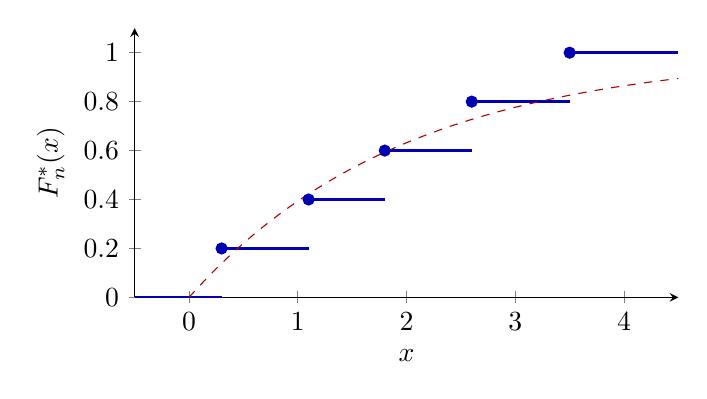
\begin{tikzpicture}
    \begin{axis}[
      width=0.7\textwidth, height=5cm,
      xmin=-0.5, xmax=4.5, ymin=0, ymax=1.1,
      axis lines=left, xlabel={$x$}, ylabel={$F_n^*(x)$},
      ytick={0, 0.2, 0.4, 0.6, 0.8, 1},
    ]
      % выборка: 0.3, 1.1, 1.8, 2.6, 3.5 (n = 5)
      \addplot[very thick, blue!70!black, domain=-0.5:0.3] {0};
      \addplot[very thick, blue!70!black, domain=0.3:1.1] {0.2};
      \addplot[very thick, blue!70!black, domain=1.1:1.8] {0.4};
      \addplot[very thick, blue!70!black, domain=1.8:2.6] {0.6};
      \addplot[very thick, blue!70!black, domain=2.6:3.5] {0.8};
      \addplot[very thick, blue!70!black, domain=3.5:4.5] {1};
      \addplot[only marks, mark=*, blue!70!black]
        coordinates {(0.3,0.2) (1.1,0.4) (1.8,0.6) (2.6,0.8) (3.5,1)};
      \addplot[dashed, red!70!black, domain=0:4.5, samples=100] {1 - exp(-x/2)};
    \end{axis}
  \end{tikzpicture}
  \caption{Эмпирическая функция распределения ($n = 5$)
           и истинная функция распределения $\Exp(1/2)$ (пунктир).}
  \label{tpl:ecdf}
\end{figure}

\subsection{Типографика}

% ~        неразрывный пробел: «на~$\R$», «по~\cref{...}»
% ~---     тире в тексте: «$X$~--- выборка»
% --       короткое тире в диапазонах и двойных фамилиях: «Гливенко--Кантелли», «1--5»
% т.\,е.   тонкий пробел в сокращениях
% \medskip, \bigskip   вертикальный отступ между блоками
% \emph{}  выделение (курсив) — для вводимых терминов
\emph{Термин}~--- выделение; «Гливенко--Кантелли»; страницы 1--5; т.\,е.
.
%
%  Новая лекция: скопируйте этот файл в lectures/lecNN.tex, удалите лишнее,
%  замените метки tpl:... на свои (например, lec03:...).
% =====================================================================
%  Лекция NN. <Тема>
%  Дата: ГГГГ-ММ-ДД
% =====================================================================

% Короткое название в [ ] попадает в оглавление и закладки PDF,
% полное — в заголовок на странице. Если название короткое, [ ] не нужны.
\section[Шаблон лекции]{Шаблон лекции: все возможности конфига}
\label{tpl:lecture}

\subsection{Окружения}

% ---------- Нумерованные окружения (общий счётчик внутри лекции) ----------

\begin{definition}
  \emph{Статистикой} называется любая борелевская функция от выборки.
\end{definition}

% Название в [ ] печатается жирным рядом с номером.
\begin{theorem}[Гливенко--Кантелли]
  \label{tpl:glivenko}
  $\sup_{x \in \R} \abs{F_n^*(x) - F(x)} \toas 0$ \textup{при} $n \to \infty$.
\end{theorem}

\begin{lemma}
  \label{tpl:lemma}
  Если $\xi_n \toas \xi$, то $\xi_n \toP \xi$.
\end{lemma}

\begin{proposition}
  \label{tpl:xbar}
  Если $\E X_1 = \mu$ конечно, то $\Xbar \toas \mu$.
\end{proposition}

\begin{proof}
  Это усиленный закон больших чисел.
\end{proof}

\begin{corollary}
  $\Xbar \toP \mu$ (по лемме~\ref{tpl:lemma}).
\end{corollary}

\begin{example}
  Если $X_i \iid \Bern(p)$, то $\Xbar \toas p$.
\end{example}

\begin{exercise}
  Докажите, что $\E S^2 = \frac{n-1}{n}\,\sigma^2$.
\end{exercise}

% ---------- Ненумерованные ----------

\begin{remark}
  Замечание: курсивный заголовок, без номера.
\end{remark}

\begin{note}
  Примечание: то же, что замечание, другое слово.
\end{note}

% ---------- Плашки ----------

% Напоминание уже известного (серое, без номера). Заголовок можно сменить:
% \begin{reminder}[Из теории вероятностей]
\begin{reminder}
  Функция $f \colon \R^n \to \R^m$ называется \emph{борелевской}, если
  $f^{-1}(B) \in \mathcal{B}(\R^n)$ для любого $B \in \mathcal{B}(\R^m)$.
\end{reminder}

% Рамка для главного итога/формулы (синяя). Заголовок необязателен.
\begin{keybox}[Итог]
  $\Xbar$~--- несмещённая и сильно состоятельная оценка $\mu$.
\end{keybox}

% Доказательство, которое заканчивается выносной формулой:
% \qedhere ставит квадратик на строке формулы, а не ниже.
\begin{proof}[Доказательство утверждения~\ref{tpl:xbar}]
  По линейности матожидания
  \[
    \E \Xbar = \frac1n \sum_{i=1}^n \E X_i = \mu. \qedhere
  \]
\end{proof}

\subsection{Формулы}

% Строчная формула: $...$.  Выносная без номера: \[ ... \].
Строчная формула $\xi \colon \Omega \to \R$ и выносная без номера:
\[
  \P_\xi\bigl((-\infty, x]\bigr) = F(x).
\]

% С номером (номер вида (NN.k)) и меткой для ссылки:
Выносная с номером:
\begin{equation}
  \label{tpl:eq:mean}
  \Xbar = \frac{1}{n} \sum_{i=1}^{n} X_i.
\end{equation}

% Несколько строк, выровненных по & (обычно перед =). Без номеров — align*,
% с номерами — align (тогда \notag убирает номер у отдельной строки).
Несколько строк с выравниванием:
\begin{align}
  \E S^2 &= \E X_1^2 - \E \Xbar^2 \notag \\
         &= \frac{n-1}{n}\,\sigma^2. \label{tpl:eq:s2}
\end{align}

% Несколько строк по центру, без выравнивания:
\begin{gather*}
  \nu_1 + \ldots + \nu_m = n, \\
  h_i = \frac{\nu_i}{n l_i}.
\end{gather*}

% Кусочная функция. Дроби в cases маленькие; для крупных — dcases.
Кусочная функция:
\[
  \Ind{x \in A} =
  \begin{cases}
    1, & \text{если } x \in A, \\
    0, & \text{иначе}.
  \end{cases}
\]

\subsection{Ссылки}

% \cref сам подставляет слово: «теорема», «утверждение», «лекция», «рис.»...
% но ТОЛЬКО в именительном падеже. Для других падежей пишите слово сами
% и ставьте \ref (только номер): «по теореме~\ref{...}», «из леммы~\ref{...}».
% Формулы: \cref{eq} даёт «(3.1)» — подходит в любом падеже.
См. \cref{tpl:glivenko}; \cref{tpl:xbar}; \cref{tpl:ecdf}.
По теореме~\ref{tpl:glivenko} эмпирическая функция распределения сходится
равномерно. Из формул \cref{tpl:eq:mean} и~\cref{tpl:eq:s2} следует\ldots{}
Ссылка на другую лекцию: см.~\cref{lec:01}.

\subsection{Макросы обозначений}

% Полный список — в preamble/macros.tex и в таблице notation.tex.
\begin{itemize}
  \item Множества: $\R$, $\N$, $\Z$, $\mathcal{B}(\R)$.
  \item Моменты: $\P(A)$, $\E X$, $\D X$, $\Var X$, $\cov(X, Y)$, $\corr(X, Y)$, $\Ind{A}$.
  \item Модель: $\Pt$, $\Et$, $\Dt$, $\Th$, $\sample$, $\Xbar$, $\est\theta$, $X_i \iid F$.
  \item Эмпирические: $\Pemp(B)$, $F_n^*(x)$.
  \item Сходимости: $\toas$, $\toP$, $\tod$, $\toLp{2}$.
  \item Распределения: $\Norm(\mu, \sigma^2)$, $\Bern(p)$, $\Bin(n, p)$,
        $\Pois(\lambda)$, $\Exp(\lambda)$, $\Unif[a, b]$.
  \item Прочее: $a \eqdef b$, $\argmax_\theta L(\theta)$, $\abs{x}$,
        $\epsilon$ (это $\varepsilon$), $\phi$ (это $\varphi$),
        $\le$ и $\ge$ (наклонные).
\end{itemize}

\subsection{Списки}

% Нумерованный список. Метки можно менять: \begin{enumerate}[label=(\alph*)]
\begin{enumerate}
  \item несмещённость;
  \item состоятельность.
\end{enumerate}

\begin{enumerate}[label=(\alph*)]
  \item первый пункт;
  \item второй пункт.
\end{enumerate}

\subsection{Рисунки}

% График средствами pgfplots. Картинку из файла можно вставить так:
%   \includegraphics[width=0.6\textwidth]{имя_файла}   % файл лежит в figures/
\begin{figure}[h]
  \centering
  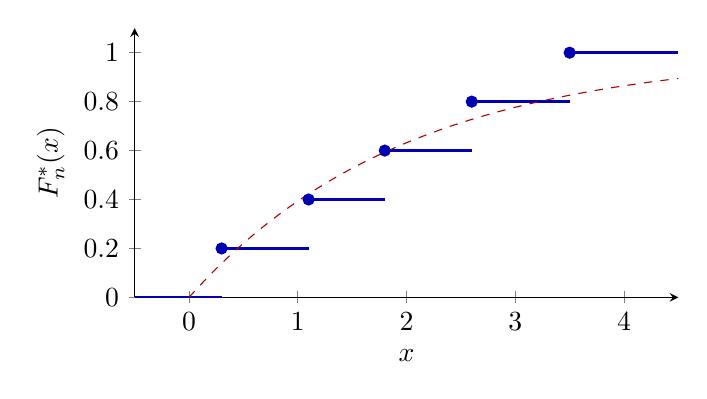
\begin{tikzpicture}
    \begin{axis}[
      width=0.7\textwidth, height=5cm,
      xmin=-0.5, xmax=4.5, ymin=0, ymax=1.1,
      axis lines=left, xlabel={$x$}, ylabel={$F_n^*(x)$},
      ytick={0, 0.2, 0.4, 0.6, 0.8, 1},
    ]
      % выборка: 0.3, 1.1, 1.8, 2.6, 3.5 (n = 5)
      \addplot[very thick, blue!70!black, domain=-0.5:0.3] {0};
      \addplot[very thick, blue!70!black, domain=0.3:1.1] {0.2};
      \addplot[very thick, blue!70!black, domain=1.1:1.8] {0.4};
      \addplot[very thick, blue!70!black, domain=1.8:2.6] {0.6};
      \addplot[very thick, blue!70!black, domain=2.6:3.5] {0.8};
      \addplot[very thick, blue!70!black, domain=3.5:4.5] {1};
      \addplot[only marks, mark=*, blue!70!black]
        coordinates {(0.3,0.2) (1.1,0.4) (1.8,0.6) (2.6,0.8) (3.5,1)};
      \addplot[dashed, red!70!black, domain=0:4.5, samples=100] {1 - exp(-x/2)};
    \end{axis}
  \end{tikzpicture}
  \caption{Эмпирическая функция распределения ($n = 5$)
           и истинная функция распределения $\Exp(1/2)$ (пунктир).}
  \label{tpl:ecdf}
\end{figure}

\subsection{Типографика}

% ~        неразрывный пробел: «на~$\R$», «по~\cref{...}»
% ~---     тире в тексте: «$X$~--- выборка»
% --       короткое тире в диапазонах и двойных фамилиях: «Гливенко--Кантелли», «1--5»
% т.\,е.   тонкий пробел в сокращениях
% \medskip, \bigskip   вертикальный отступ между блоками
% \emph{}  выделение (курсив) — для вводимых терминов
\emph{Термин}~--- выделение; «Гливенко--Кантелли»; страницы 1--5; т.\,е.
.
%
%  Новая лекция: скопируйте этот файл в lectures/lecNN.tex, удалите лишнее,
%  замените метки tpl:... на свои (например, lec03:...).
% =====================================================================
%  Лекция NN. <Тема>
%  Дата: ГГГГ-ММ-ДД
% =====================================================================

% Короткое название в [ ] попадает в оглавление и закладки PDF,
% полное — в заголовок на странице. Если название короткое, [ ] не нужны.
\section[Шаблон лекции]{Шаблон лекции: все возможности конфига}
\label{tpl:lecture}

\subsection{Окружения}

% ---------- Нумерованные окружения (общий счётчик внутри лекции) ----------

\begin{definition}
  \emph{Статистикой} называется любая борелевская функция от выборки.
\end{definition}

% Название в [ ] печатается жирным рядом с номером.
\begin{theorem}[Гливенко--Кантелли]
  \label{tpl:glivenko}
  $\sup_{x \in \R} \abs{F_n^*(x) - F(x)} \toas 0$ \textup{при} $n \to \infty$.
\end{theorem}

\begin{lemma}
  \label{tpl:lemma}
  Если $\xi_n \toas \xi$, то $\xi_n \toP \xi$.
\end{lemma}

\begin{proposition}
  \label{tpl:xbar}
  Если $\E X_1 = \mu$ конечно, то $\Xbar \toas \mu$.
\end{proposition}

\begin{proof}
  Это усиленный закон больших чисел.
\end{proof}

\begin{corollary}
  $\Xbar \toP \mu$ (по лемме~\ref{tpl:lemma}).
\end{corollary}

\begin{example}
  Если $X_i \iid \Bern(p)$, то $\Xbar \toas p$.
\end{example}

\begin{exercise}
  Докажите, что $\E S^2 = \frac{n-1}{n}\,\sigma^2$.
\end{exercise}

% ---------- Ненумерованные ----------

\begin{remark}
  Замечание: курсивный заголовок, без номера.
\end{remark}

\begin{note}
  Примечание: то же, что замечание, другое слово.
\end{note}

% ---------- Плашки ----------

% Напоминание уже известного (серое, без номера). Заголовок можно сменить:
% \begin{reminder}[Из теории вероятностей]
\begin{reminder}
  Функция $f \colon \R^n \to \R^m$ называется \emph{борелевской}, если
  $f^{-1}(B) \in \mathcal{B}(\R^n)$ для любого $B \in \mathcal{B}(\R^m)$.
\end{reminder}

% Рамка для главного итога/формулы (синяя). Заголовок необязателен.
\begin{keybox}[Итог]
  $\Xbar$~--- несмещённая и сильно состоятельная оценка $\mu$.
\end{keybox}

% Доказательство, которое заканчивается выносной формулой:
% \qedhere ставит квадратик на строке формулы, а не ниже.
\begin{proof}[Доказательство утверждения~\ref{tpl:xbar}]
  По линейности матожидания
  \[
    \E \Xbar = \frac1n \sum_{i=1}^n \E X_i = \mu. \qedhere
  \]
\end{proof}

\subsection{Формулы}

% Строчная формула: $...$.  Выносная без номера: \[ ... \].
Строчная формула $\xi \colon \Omega \to \R$ и выносная без номера:
\[
  \P_\xi\bigl((-\infty, x]\bigr) = F(x).
\]

% С номером (номер вида (NN.k)) и меткой для ссылки:
Выносная с номером:
\begin{equation}
  \label{tpl:eq:mean}
  \Xbar = \frac{1}{n} \sum_{i=1}^{n} X_i.
\end{equation}

% Несколько строк, выровненных по & (обычно перед =). Без номеров — align*,
% с номерами — align (тогда \notag убирает номер у отдельной строки).
Несколько строк с выравниванием:
\begin{align}
  \E S^2 &= \E X_1^2 - \E \Xbar^2 \notag \\
         &= \frac{n-1}{n}\,\sigma^2. \label{tpl:eq:s2}
\end{align}

% Несколько строк по центру, без выравнивания:
\begin{gather*}
  \nu_1 + \ldots + \nu_m = n, \\
  h_i = \frac{\nu_i}{n l_i}.
\end{gather*}

% Кусочная функция. Дроби в cases маленькие; для крупных — dcases.
Кусочная функция:
\[
  \Ind{x \in A} =
  \begin{cases}
    1, & \text{если } x \in A, \\
    0, & \text{иначе}.
  \end{cases}
\]

\subsection{Ссылки}

% \cref сам подставляет слово: «теорема», «утверждение», «лекция», «рис.»...
% но ТОЛЬКО в именительном падеже. Для других падежей пишите слово сами
% и ставьте \ref (только номер): «по теореме~\ref{...}», «из леммы~\ref{...}».
% Формулы: \cref{eq} даёт «(3.1)» — подходит в любом падеже.
См. \cref{tpl:glivenko}; \cref{tpl:xbar}; \cref{tpl:ecdf}.
По теореме~\ref{tpl:glivenko} эмпирическая функция распределения сходится
равномерно. Из формул \cref{tpl:eq:mean} и~\cref{tpl:eq:s2} следует\ldots{}
Ссылка на другую лекцию: см.~\cref{lec:01}.

\subsection{Макросы обозначений}

% Полный список — в preamble/macros.tex и в таблице notation.tex.
\begin{itemize}
  \item Множества: $\R$, $\N$, $\Z$, $\mathcal{B}(\R)$.
  \item Моменты: $\P(A)$, $\E X$, $\D X$, $\Var X$, $\cov(X, Y)$, $\corr(X, Y)$, $\Ind{A}$.
  \item Модель: $\Pt$, $\Et$, $\Dt$, $\Th$, $\sample$, $\Xbar$, $\est\theta$, $X_i \iid F$.
  \item Эмпирические: $\Pemp(B)$, $F_n^*(x)$.
  \item Сходимости: $\toas$, $\toP$, $\tod$, $\toLp{2}$.
  \item Распределения: $\Norm(\mu, \sigma^2)$, $\Bern(p)$, $\Bin(n, p)$,
        $\Pois(\lambda)$, $\Exp(\lambda)$, $\Unif[a, b]$.
  \item Прочее: $a \eqdef b$, $\argmax_\theta L(\theta)$, $\abs{x}$,
        $\epsilon$ (это $\varepsilon$), $\phi$ (это $\varphi$),
        $\le$ и $\ge$ (наклонные).
\end{itemize}

\subsection{Списки}

% Нумерованный список. Метки можно менять: \begin{enumerate}[label=(\alph*)]
\begin{enumerate}
  \item несмещённость;
  \item состоятельность.
\end{enumerate}

\begin{enumerate}[label=(\alph*)]
  \item первый пункт;
  \item второй пункт.
\end{enumerate}

\subsection{Рисунки}

% График средствами pgfplots. Картинку из файла можно вставить так:
%   \includegraphics[width=0.6\textwidth]{имя_файла}   % файл лежит в figures/
\begin{figure}[h]
  \centering
  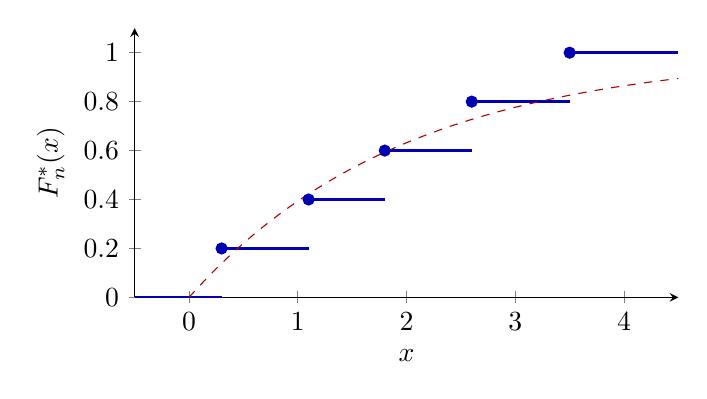
\begin{tikzpicture}
    \begin{axis}[
      width=0.7\textwidth, height=5cm,
      xmin=-0.5, xmax=4.5, ymin=0, ymax=1.1,
      axis lines=left, xlabel={$x$}, ylabel={$F_n^*(x)$},
      ytick={0, 0.2, 0.4, 0.6, 0.8, 1},
    ]
      % выборка: 0.3, 1.1, 1.8, 2.6, 3.5 (n = 5)
      \addplot[very thick, blue!70!black, domain=-0.5:0.3] {0};
      \addplot[very thick, blue!70!black, domain=0.3:1.1] {0.2};
      \addplot[very thick, blue!70!black, domain=1.1:1.8] {0.4};
      \addplot[very thick, blue!70!black, domain=1.8:2.6] {0.6};
      \addplot[very thick, blue!70!black, domain=2.6:3.5] {0.8};
      \addplot[very thick, blue!70!black, domain=3.5:4.5] {1};
      \addplot[only marks, mark=*, blue!70!black]
        coordinates {(0.3,0.2) (1.1,0.4) (1.8,0.6) (2.6,0.8) (3.5,1)};
      \addplot[dashed, red!70!black, domain=0:4.5, samples=100] {1 - exp(-x/2)};
    \end{axis}
  \end{tikzpicture}
  \caption{Эмпирическая функция распределения ($n = 5$)
           и истинная функция распределения $\Exp(1/2)$ (пунктир).}
  \label{tpl:ecdf}
\end{figure}

\subsection{Типографика}

% ~        неразрывный пробел: «на~$\R$», «по~\cref{...}»
% ~---     тире в тексте: «$X$~--- выборка»
% --       короткое тире в диапазонах и двойных фамилиях: «Гливенко--Кантелли», «1--5»
% т.\,е.   тонкий пробел в сокращениях
% \medskip, \bigskip   вертикальный отступ между блоками
% \emph{}  выделение (курсив) — для вводимых терминов
\emph{Термин}~--- выделение; «Гливенко--Кантелли»; страницы 1--5; т.\,е.
.
%
%  Новая лекция: скопируйте этот файл в lectures/lecNN.tex, удалите лишнее,
%  замените метки tpl:... на свои (например, lec03:...).
% =====================================================================
%  Лекция NN. <Тема>
%  Дата: ГГГГ-ММ-ДД
% =====================================================================

% Короткое название в [ ] попадает в оглавление и закладки PDF,
% полное — в заголовок на странице. Если название короткое, [ ] не нужны.
\section[Шаблон лекции]{Шаблон лекции: все возможности конфига}
\label{tpl:lecture}

\subsection{Окружения}

% ---------- Нумерованные окружения (общий счётчик внутри лекции) ----------

\begin{definition}
  \emph{Статистикой} называется любая борелевская функция от выборки.
\end{definition}

% Название в [ ] печатается жирным рядом с номером.
\begin{theorem}[Гливенко--Кантелли]
  \label{tpl:glivenko}
  $\sup_{x \in \R} \abs{F_n^*(x) - F(x)} \toas 0$ \textup{при} $n \to \infty$.
\end{theorem}

\begin{lemma}
  \label{tpl:lemma}
  Если $\xi_n \toas \xi$, то $\xi_n \toP \xi$.
\end{lemma}

\begin{proposition}
  \label{tpl:xbar}
  Если $\E X_1 = \mu$ конечно, то $\Xbar \toas \mu$.
\end{proposition}

\begin{proof}
  Это усиленный закон больших чисел.
\end{proof}

\begin{corollary}
  $\Xbar \toP \mu$ (по лемме~\ref{tpl:lemma}).
\end{corollary}

\begin{example}
  Если $X_i \iid \Bern(p)$, то $\Xbar \toas p$.
\end{example}

\begin{exercise}
  Докажите, что $\E S^2 = \frac{n-1}{n}\,\sigma^2$.
\end{exercise}

% ---------- Ненумерованные ----------

\begin{remark}
  Замечание: курсивный заголовок, без номера.
\end{remark}

\begin{note}
  Примечание: то же, что замечание, другое слово.
\end{note}

% ---------- Плашки ----------

% Напоминание уже известного (серое, без номера). Заголовок можно сменить:
% \begin{reminder}[Из теории вероятностей]
\begin{reminder}
  Функция $f \colon \R^n \to \R^m$ называется \emph{борелевской}, если
  $f^{-1}(B) \in \mathcal{B}(\R^n)$ для любого $B \in \mathcal{B}(\R^m)$.
\end{reminder}

% Рамка для главного итога/формулы (синяя). Заголовок необязателен.
\begin{keybox}[Итог]
  $\Xbar$~--- несмещённая и сильно состоятельная оценка $\mu$.
\end{keybox}

% Доказательство, которое заканчивается выносной формулой:
% \qedhere ставит квадратик на строке формулы, а не ниже.
\begin{proof}[Доказательство утверждения~\ref{tpl:xbar}]
  По линейности матожидания
  \[
    \E \Xbar = \frac1n \sum_{i=1}^n \E X_i = \mu. \qedhere
  \]
\end{proof}

\subsection{Формулы}

% Строчная формула: $...$.  Выносная без номера: \[ ... \].
Строчная формула $\xi \colon \Omega \to \R$ и выносная без номера:
\[
  \P_\xi\bigl((-\infty, x]\bigr) = F(x).
\]

% С номером (номер вида (NN.k)) и меткой для ссылки:
Выносная с номером:
\begin{equation}
  \label{tpl:eq:mean}
  \Xbar = \frac{1}{n} \sum_{i=1}^{n} X_i.
\end{equation}

% Несколько строк, выровненных по & (обычно перед =). Без номеров — align*,
% с номерами — align (тогда \notag убирает номер у отдельной строки).
Несколько строк с выравниванием:
\begin{align}
  \E S^2 &= \E X_1^2 - \E \Xbar^2 \notag \\
         &= \frac{n-1}{n}\,\sigma^2. \label{tpl:eq:s2}
\end{align}

% Несколько строк по центру, без выравнивания:
\begin{gather*}
  \nu_1 + \ldots + \nu_m = n, \\
  h_i = \frac{\nu_i}{n l_i}.
\end{gather*}

% Кусочная функция. Дроби в cases маленькие; для крупных — dcases.
Кусочная функция:
\[
  \Ind{x \in A} =
  \begin{cases}
    1, & \text{если } x \in A, \\
    0, & \text{иначе}.
  \end{cases}
\]

\subsection{Ссылки}

% \cref сам подставляет слово: «теорема», «утверждение», «лекция», «рис.»...
% но ТОЛЬКО в именительном падеже. Для других падежей пишите слово сами
% и ставьте \ref (только номер): «по теореме~\ref{...}», «из леммы~\ref{...}».
% Формулы: \cref{eq} даёт «(3.1)» — подходит в любом падеже.
См. \cref{tpl:glivenko}; \cref{tpl:xbar}; \cref{tpl:ecdf}.
По теореме~\ref{tpl:glivenko} эмпирическая функция распределения сходится
равномерно. Из формул \cref{tpl:eq:mean} и~\cref{tpl:eq:s2} следует\ldots{}
Ссылка на другую лекцию: см.~\cref{lec:01}.

\subsection{Макросы обозначений}

% Полный список — в preamble/macros.tex и в таблице notation.tex.
\begin{itemize}
  \item Множества: $\R$, $\N$, $\Z$, $\mathcal{B}(\R)$.
  \item Моменты: $\P(A)$, $\E X$, $\D X$, $\Var X$, $\cov(X, Y)$, $\corr(X, Y)$, $\Ind{A}$.
  \item Модель: $\Pt$, $\Et$, $\Dt$, $\Th$, $\sample$, $\Xbar$, $\est\theta$, $X_i \iid F$.
  \item Эмпирические: $\Pemp(B)$, $F_n^*(x)$.
  \item Сходимости: $\toas$, $\toP$, $\tod$, $\toLp{2}$.
  \item Распределения: $\Norm(\mu, \sigma^2)$, $\Bern(p)$, $\Bin(n, p)$,
        $\Pois(\lambda)$, $\Exp(\lambda)$, $\Unif[a, b]$.
  \item Прочее: $a \eqdef b$, $\argmax_\theta L(\theta)$, $\abs{x}$,
        $\epsilon$ (это $\varepsilon$), $\phi$ (это $\varphi$),
        $\le$ и $\ge$ (наклонные).
\end{itemize}

\subsection{Списки}

% Нумерованный список. Метки можно менять: \begin{enumerate}[label=(\alph*)]
\begin{enumerate}
  \item несмещённость;
  \item состоятельность.
\end{enumerate}

\begin{enumerate}[label=(\alph*)]
  \item первый пункт;
  \item второй пункт.
\end{enumerate}

\subsection{Рисунки}

% График средствами pgfplots. Картинку из файла можно вставить так:
%   \includegraphics[width=0.6\textwidth]{имя_файла}   % файл лежит в figures/
\begin{figure}[h]
  \centering
  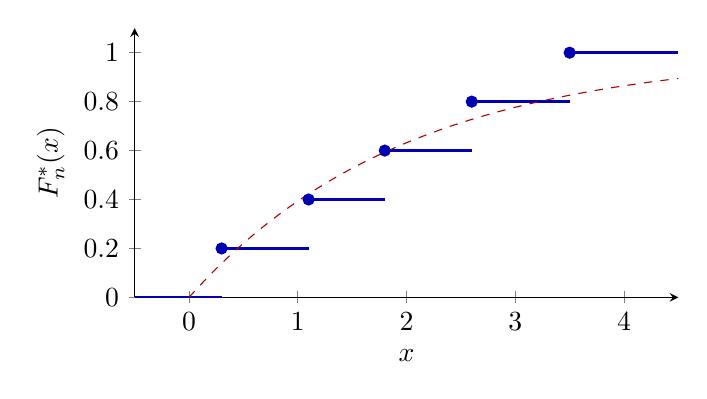
\begin{tikzpicture}
    \begin{axis}[
      width=0.7\textwidth, height=5cm,
      xmin=-0.5, xmax=4.5, ymin=0, ymax=1.1,
      axis lines=left, xlabel={$x$}, ylabel={$F_n^*(x)$},
      ytick={0, 0.2, 0.4, 0.6, 0.8, 1},
    ]
      % выборка: 0.3, 1.1, 1.8, 2.6, 3.5 (n = 5)
      \addplot[very thick, blue!70!black, domain=-0.5:0.3] {0};
      \addplot[very thick, blue!70!black, domain=0.3:1.1] {0.2};
      \addplot[very thick, blue!70!black, domain=1.1:1.8] {0.4};
      \addplot[very thick, blue!70!black, domain=1.8:2.6] {0.6};
      \addplot[very thick, blue!70!black, domain=2.6:3.5] {0.8};
      \addplot[very thick, blue!70!black, domain=3.5:4.5] {1};
      \addplot[only marks, mark=*, blue!70!black]
        coordinates {(0.3,0.2) (1.1,0.4) (1.8,0.6) (2.6,0.8) (3.5,1)};
      \addplot[dashed, red!70!black, domain=0:4.5, samples=100] {1 - exp(-x/2)};
    \end{axis}
  \end{tikzpicture}
  \caption{Эмпирическая функция распределения ($n = 5$)
           и истинная функция распределения $\Exp(1/2)$ (пунктир).}
  \label{tpl:ecdf}
\end{figure}

\subsection{Типографика}

% ~        неразрывный пробел: «на~$\R$», «по~\cref{...}»
% ~---     тире в тексте: «$X$~--- выборка»
% --       короткое тире в диапазонах и двойных фамилиях: «Гливенко--Кантелли», «1--5»
% т.\,е.   тонкий пробел в сокращениях
% \medskip, \bigskip   вертикальный отступ между блоками
% \emph{}  выделение (курсив) — для вводимых терминов
\emph{Термин}~--- выделение; «Гливенко--Кантелли»; страницы 1--5; т.\,е.
